\documentclass[12pt,letterpaper,spanish]{article}
\usepackage[utf8]{inputenc}
\usepackage[spanish]{babel}
\usepackage{amsmath}
\usepackage{amsfonts}
\usepackage{amssymb}
\usepackage{caption}
\usepackage{graphicx}%para insertar figuras
\usepackage{natbib}%necesario para que las citas aparezcan segun el formato APA o Elsevier-Harvard
\usepackage[left=1.5in,right=1in,top=1in,bottom=1in]{geometry}
\usepackage[all]{nowidow}%para evitar parrafos con lineas viudas o lineas huerfanas
\usepackage[T1]{fontenc}
\usepackage{mathptmx}
\usepackage{setspace}
\doublespacing
\usepackage{titlesec}
\titleformat{\section}[block]{\Large\bfseries\filcenter}{}{1em}{}
%\titleformat{\section}[block]{\color{blue}\Large\bfseries\filcenter}
%\usepackage{apacite}
\usepackage{enumerate} %para enumerar lista de objetivos
\usepackage{graphicx} %graficos y fuguras
\usepackage{siunitx} %coordenada
\usepackage{multirow} %para tablas
\usepackage{array} %para confg colunnas
\newcolumntype{M}[1]{>{\centering\arraybackslash}m{#1}}
\usepackage[euler]{textgreek}
\usepackage{fancyhdr} %para editar la posicion del numero de las paginas
\pagestyle{fancy}
%\fancyhead[RO,LE]{\thepage}
\renewcommand{\headrulewidth}{0pt} % elimina linea en la numeracion del comando anterior
\lhead{}
\rhead{\thepage}
\cfoot{} %elimina numeracion por defecto al pie de pagina

\title{anteproyecto}
\date{}
\usepackage[hang]{footmisc} %un paquete para habilitar las sangrias francesas
\setlength\footnotemargin{10pt} %para que las notas al pie se vean en sangria francesa
\setlength{\parskip}{1em}


\begin{document}
\thispagestyle{empty}
\begin{center}

\vspace*{0.5cm}

Universidad Autónoma de Santo Domingo\\
Facultad de Ciencias\\
Escuela de Biología

\vspace{1.0cm}
Distribución y diversidad de náyades de odonatos (Insecta: Odonata) en la Reserva Científica Ébano Verde: relación con litología, hidrografía y cobertura boscosa

\vspace{0.5cm}
\text{Propuesta de tesis para optar por el título de Licenciatura en Biología}

\vspace{0.5cm}
Sustentante\\
Br. América Sánchez Rosario

\vspace{0.5cm}
Matrícula\\
DF-9295

\vspace{0.5cm}
Asesores\\
Ruth H. Bastardo L., M Sc.\\
José Ramón Martínez Batlle, Ph.D.

\vspace{0.5cm}
Santo Domingo, D. N.\\
10 agosto de 2018

\end{center}





\newpage
\section*{INTRODUCCIÓN}

La región Caribe es considerada uno de los lugares más importantes para la biodiversidad a nivel global \citep{myers2000biodiversity}. La isla Española, cuya parte oriental pertenece a República Dominicana, presenta una singular diversidad de hábitats y especies, tanto por su compleja historia geológica \citep{perez2010geologia} como por su paleogeografía \citep{graham2003geohistory, pindell2009tectonic}, contribuyendo así a la variedad y complejidad de sus múltiples ambientes terrestres, acuáticos, costeros y marinos, y a la  biota asociada a los mismos \citep{fern2015reservas}.

La biodiversidad dominicana está sometida a múltiples amenazas \citep{fern2015reservas, kennedy20064000, myers2004evaluacion}. Muchos factores influyen en la pérdida de biodiversidad, la fragmentación de los hábitats producto de perturbaciones naturales o antropización en muchas áreas de la isla son ejemplo de ello. Estudios que contribuyan a mejorar la falta de información en cuanto a aspectos ecológicos, inventarios, abundancia y distribución de las especies, son necesarios.

Un indicador de la pérdida de biodiversidad es la reducción de la cobertura boscosa. Estudios demuestran que entre los años 2000 y 2012 la pérdida de cobertura ha sido significativa en La Española \citep{hansen2013high}, siendo una de las principales causas los incendios forestales. Diversas áreas del país, como los parques nacionales Sierra de Bahoruco, José del Carmen Ramírez y Valle Nuevo \citep{myers2004evaluacion} han sido afectadas por los mismos. Una evaluación que he realizado con imágenes de satélite para los fines de esta investigación, detectó que al menos un 5\% del bosque de la Reserva Científica Ébano Verde (en lo adelante, RCEV) ha resultado afectado por incendios forestales en las últimas décadas. 

Un caso de pérdida de diversidad para la RCEV fue estudiado por \citet{slocum2000vegetacion}, quienes compararon la diversidad florística de áreas dominadas por helechos (especialmente Dicranopteris pectinata) y bosques ribereños en un área de montaña tropical de la reserva, demostrando que los helechos pueden limitar la diversidad y densidad de plantas leñosas, debido a la competencia por el espacio y a la restricción en la dispersión de semillas. \citet{may2000respuesta} también examinó la respuesta de la vegetación en un ''calimetal'' de Dicranopteris pectinata después de un fuego en la RCEV. Estos estudios permitieron que \citet{navarro2006restauracion} diseñaran un plan de acción para la restauración de las especies nativas en los helechales de la reserva.

La RCEV ha sido un espacio de alto interés para el estudio de la vegetación, mas no así para la fauna de invertebrados. Sus elevaciones y clima, producto de las precipitaciones frecuentes, contribuyen al caudal en los nacimientos de varios ríos que abastecen las necesidades de agua de los pueblos de Constanza y Jarabacoa. Es por esto que consideramos la reserva como un lugar idóneo para el estudio de la fauna, especialmente insectos.

Varios estudios en la RCEV han sido enfocados hacia la respuesta o interacciones entre plantas a perturbaciones \citep{may2000respuesta, slocum2000vegetacion} y otros sobre musgos \citep{jimenez2011diversidad} y hongos \citep{quirico2004basidiomycetes}. Sin embargo, se han realizado pocas aportaciones sobre los  invertebrados, específicamente insectos, siendo el trabajo más reciente la lista de especies publicada  por \citet{perez2015entomofauna}.

Los odonatos (Insecta: Odonata), conocidos comúnmente como caballitos, helicópteros, libélulas o pinchitos en el caso de los Zygoptera (caballitos como nombre común para los dominicanos), son insectos hemimetábolos que viven asociados a cuerpos de agua, los cuales necesitan en su primera etapa de desarrollo (náyade). Es uno de los órdenes mejor conocidos a nivel mundial, muy abundantes y de fácil identificación en el campo \citep{ramirez2010capitulo}. Aunque aún existen vacíos en varios aspectos, en la isla Española según \citet{bastardo2017estado}, la taxonomía y distribución de este grupo ha sido bien estudiada. Su asociación con ecosistemas acuáticos, los hace aptos para el estudio de la biodiversidad.

En República Dominicana no se ha encontrado un registro sobre la posible asociación de los odonatos con factores de tipo litológico, hidrográfico y cobertura boscosa. Partiendo del hecho de que el tipo de roca influye en el ecosistema, se analizará su posible asociación con el grupo de estudio.

En esta investigación se propone, determinar si la composición y estructura de las poblaciones de náyades de odonatos de la RCEV varía según los cambios en los estratos litología (tipo de roca), hidrografía (orden de red hidrográfica) y cobertura boscosa. A la combinación generada entre los estratos se le denomina subgrupo \citep{triola2009estadistica, rojas2000investigar} y estos subgrupos facilitarán el muestreo. Este conocimiento podría servir de apoyo a futuras acciones de conservación, pues cinco de las especies de odonatos presentes en la Reserva, son endémicas de la República Dominicana \citep{flint2006distribution, perez2015entomofauna}.

\newpage
\section*{ANTECEDENTES}

\citet{flint2006distribution} compilaron la información disponible sobre odonatos en una lista por provincias de la República Dominicana un total de 67 especies, de las cuales siete endémicas y ocho especies en la actualidad con Hipolestes hatuey (antes Hipolestes trinitatis) descrita por \citet{torres2015hypolestes}, las 59 restante son nativas. \citet{perez2008arthropods} en el catálogo sobre los artrópodos de La Hispaniola registró la fauna viviente, extinta o en ámbar sobre Odonata.

Otro estudio que incluye los odonatos, es el de \citet{almonte2012caracterizacion}, el cual relaciona la presencia de la cigüita del río con la abundancia y diversidad del grupo de los insectos acuáticos y otros invertebrados. Aunque en este estudio los odonatos no fueron uno de los órdenes mejor representados, nos ofrece datos de relevancia de sus depredadores.

En el análisis sobre los odonatos de la Cordillera Central de la República Dominicana, \citet{sanchez2014analisis} sugieren que la riqueza de odonatos es baja, a pesar de la gran cantidad de ríos y arroyos. En esta cordillera se encuentran 34 de las 123 áreas protegidas del país siendo la RCEV el área protegida con mayor riqueza de especies.

Otro trabajo donde se refleja la necesidad de ampliar el conocimiento sobre las libélulas dominicanas es el de \citet{sanchez2015libelulidos} sobre los Libelúlidos de la Colección Entomológica del Instituto de Investigaciones Botánicas y Zoológicas (IIBZ). Un salto importante en el registro de especímenes de esta familia (Libellulidae), la cual se encuentra dividida en dicha colección en dos periodos de colecta, 1958-1979 y 2001-2004. Al menos unas cuatro provincias del país aún no han sido exploradas y se encuentran sin ningún registro de esta familia.

Recientemente, \citep{bastardo2017estado} ofrecen una panorámica más completa sobre los insectos acuáticos incluyendo libélulas. Este trabajo refiere que pocas especies de insectos tienen algún nivel de protección legal, siendo los odonatos el segundo grupo de insectos incluidos en la Lista Roja de especies amenazadas de la UICN.

\citet{perez2015entomofauna} lista las especies de insectos conocidos para la RCEV. Los odonatos estuvieron representados por 17 especies en siete familias. A pesar de lo escrito anteriormente, no existe un trabajo previo publicado sobre los odonatos en esta área protegida, ni estudios que contemplen aspectos ecológicos y de diversidad sobre el grupo. 

\newpage
\section*{JUSTIFICACIÓN}

Los estudios sobre odonatos en la República Dominicana han sido orientados a taxonomía y distribución de especies. Factores ambientales como topografía, geología, clima, entre otros, influyen en la vegetación \citep{castillo1997estudios, may2007composicion} ofreciendo múltiples hábitats que son utilizados por especies de invertebrados, es importante analizar esta interacción. En particular la asociación de los odonatos con su ambiente, no ha sido estudiada. Este trabajo sería el primero en abordar aspectos ecológicos de este tipo.

Frecuentemente, en ecología se evalúa la asociación entre las especies y su hábitat, para lo cual se requiere de un diseño de muestreo estandarizado, orientado a dar respuesta a preguntas, así como de índices y análisis estadísticos apropiados \citep{caceres2009associations}. Por tanto el presente estudio se abordará bajo esta condición. A través del estudio de las náyades de odonatos de la RCEV, se podrían inferir asociaciones con factores del entorno, así como también si la composición de especies cambia según el tipo de sustrato sobre el cual se haya originado su ecosistema.

\newpage
\section*{OBJETIVOS}
\vspace*{1.0cm}
\subsection{Objetivo general}

Evaluar la distribución y diversidad de náyades de odonatos en la RCEV: relación con la litología, la hidrografía y la cobertura boscosa.

\subsubsection{Objetivos específicos}
\begin{enumerate}
\item Estimar la riqueza de especies por estratos
\item Analizar la diversidad alfa en los subgrupos por estratos 
\item Comparar la diversidad entre subgrupos (diversidad beta) 
\item Evaluar si existe asociación entre las especies y las variables seleccionadas
\item Determinar la distribución de especies en la reserva
\end{enumerate}

\newpage
\section*{MATERIALES Y MÉTODOS}
\subsection{Área de estudio}

La Reserva Científica Ébano Verde está ubicada en la Cordillera Central en los Municipios Constanza y Jarabacoa, Provincia La Vega \citep{ley2013202}, en las coordenadas $70^\circ 31^\prime$  y $70^\circ 35^\prime$ longitud oeste y $19^\circ 01^\prime$ y $19^\circ 06^\prime$ latitud norte. Posee un área aproximada de 23.1 km\textsuperscript{2}, la misma abarca los picos de las lomas La Golondrina, La Sal, El Col y Alto de Casabito (Fig.\ref{fig:mapaRCEV}).

\begin{figure}[h!]
\centering
  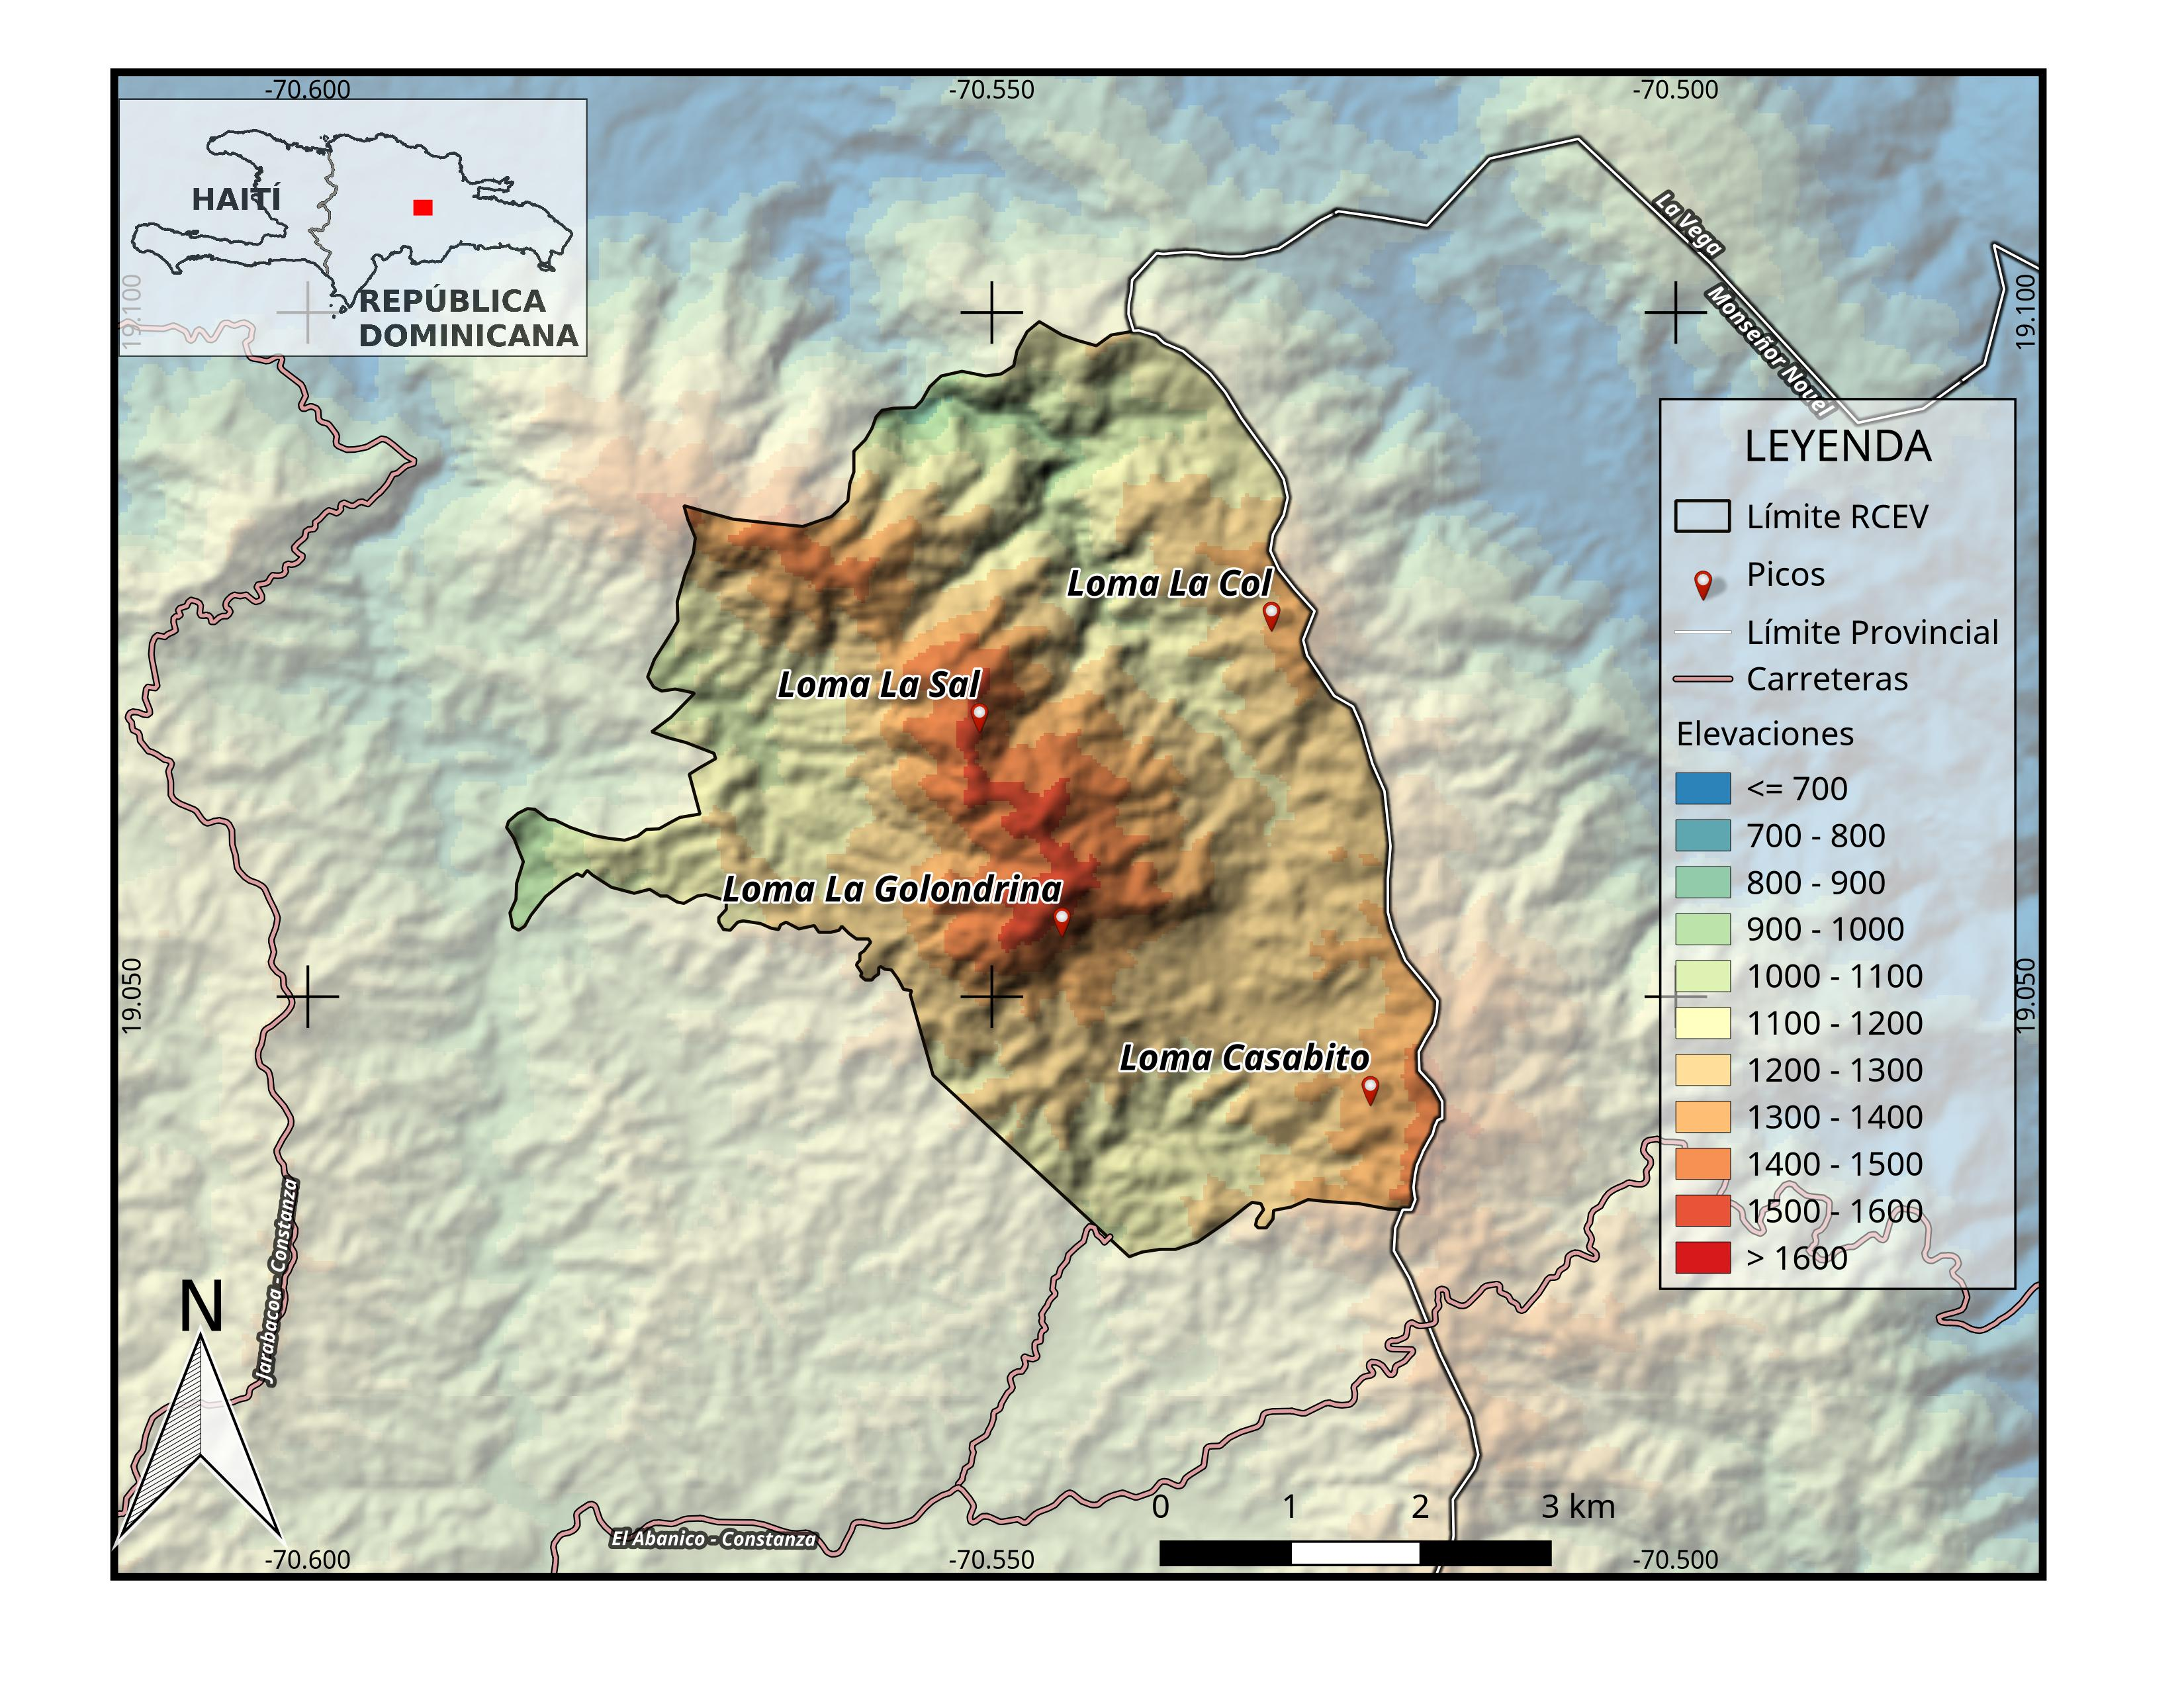
\includegraphics[width=\linewidth]{mapaRCEV.jpeg}
  \caption{Límites de la Reserva Científica Ébano Verde con sus elevaciones y picos de importancia.}
  \label{fig:mapaRCEV}
\end{figure}

El bosque nublado ocupa la mayor extensión dentro de la Reserva Científica. Las especies arbóreas más características son el palo de viento (\textit{Schefflera tremula}), la manacla (\textit{Prestoea acuminata var. montana}) y el ébano verde (\textit{Magnolia pallescens}). Según \citet{garcia1994composicion}, en la RCEV se observa un mosaico de la sucesión natural del bosque en numerosas áreas que fueron alteradas por deslizamientos de tierra, fuegos, conucos abandonados y corte para madera, en las cuales se está recuperando la vegetación nativa.

La RCEV está compuesta litológicamente en su mayoría por cuatro tipos de rocas, a saber: a) basaltos, b) leucotonalita hornblendico/biotítica, c) tobas líticas y vítreas masivas y d) tonalita hornblendica \citep{servicio2000mapageol}. Sobre estas rocas fluyen los nacimientos de los ríos Camú, Jimenoa y Jatubey, y algunos arroyos caudolosos como La Sal, Bonito y El Arroyazo \citep{fern2015reservas}.

\subsection{Selección y ubicación de los puntos de muestreo}

El diseño de muestreo aleatorio estratificado por subgrupos  \citep{krebs1989ecological, triola2009estadistica} es el más idóneo para alcanzar los objetivos propuestos y determinar si la composición y estructura de las poblaciones de odonatos en la RCEV varían según los cambios de cobertura, litología e hidrografía. En observaciones no sistemáticas sobre los odonatos en la RCEV se ha verificado variabilidad en cuanto abundancia y riqueza de especies según litología e hidrografía. Por esta razón, se reunirán capas de información geográfica, así como datos de campo preliminares sobre evidencia de esos subgrupos.

Con esta información, se estratificará considerando como subgrupos la combinación del orden de red (del inglés \textit{stream order}) de \citet{strahler1952hypsometric}, el tipo de roca y la cobertura boscosa. 

Los puntos de muestreo se ubicarán utilizando el Sistema de Información Geográfica QGIS \citep{qgis2018qgis}, R \citep{team2015r} y GRASS \citep{neteler2013open}, empleando como fuente un modelo digital de elevaciones para determinar el orden de red, y el mapa geológico escala 1:50,000 \citep{servicio2000mapageol} para delimitar el tipo de roca. Para estimar la cobertura boscosa se interpretará digitalmente una imagen de satélite Landsat \citep{nasa2014srtm1sdem} con poca cubierta de nubes.

El número de puntos por tipo de roca, orden de red hidrográfica y cobertura boscosa, será calculado en función del porcentaje de representación espacial que ocupen dichas categorías en el área, de manera que queden más representados aquellos subgrupos dominantes dentro de la clasificación por estratos.

\subsection{Trabajo de campo}

Se usarán formularios digitales diseñados para los fines y en formato XML, utilizando la herramienta XLSForm, para colectar datos con teléfono celular y almacenarlos con el programa Open Data Kit Aggregate Server, en lo adelante ODK \citep{hartung2010open}. Este diseño facilitará la recogida y manipulación de los datos, para una mayor calidad y eficiencia en el proceso.

\subsection{Colecta de especímenes}

Los especímenes serán colectados utilizando una red tipo D arrastrándola contra el sustrato y removiendo el mismo para desprender los organismos \citep{ramirez2010capitulo}. Para la colecta de individuos de la familia Gomphidae los cuales viven en los bancos de arena, se tamizarán en una malla de 250 \textmu m  \citep{mandal2008biocontrol, torralba2009estado} uno o varios volúmenes de sedimento. En el tamiz se colectarán manualmente los individuos. Los organismos colectados serán preservados en envases con alcohol etílico al 80 \% para ser transportados al laboratorio.

\subsection{Trabajo de laboratorio}

Los especímenes recolectados serán depositados en el Instituto de Investigaciones Botánicas y Zoológicas (IIBZ), donde se contarán e identificarán hasta el nivel taxonómico más bajo posible, siguiendo a \citet{needham2000dragonflies} y \citet{westfall1996damselflies}. Los organismos colectados serán  etiquetados con los datos de campo correspondientes, para luego ser incorporados en una base de datos.

\subsection{Análisis de los datos}

Se determinará si existen diferencias significativas de la diversidad alfa entre subgrupos, mediante inferencia estadística utilizando las pruebas t de Student, la de la suma de rangos de Wilcoxon, ANOVA o la de Kruskal Wallis dependiendo de la naturaleza de los datos. Se evaluará el cumplimiento de supuestos de normalidad, homogeneidad de varianzas, entre otros. Para todas las pruebas se elegirá 0.05 como nivel de significancia.

La diversidad beta se calculará utilizando el Índice de Presencia-Ausencia de Jaccard, el cual relaciona el número de especies compartidas con el número total de especies exclusivas. El uso de este índice tiene la ventaja de que hay disponible una tabla de valores significativos \citep{real1999tables}, con la que se pueden estimar si las similitudes o disimilitudes superan los valores esperados por azar para la cantidad de atributos comparados.

La asociación entre especies y las variables seleccionadas se analizarán mediante el “Índice del Valor Indicador” (IndVal) el cual evaluará el grado de fidelidad que pueda o no tener una especie a un determinado sustrato \citep{caceres2009associations}. Todos los análisis estadísticos se realizarán en el ambiente de programación R. 

\newpage
\section*{CRONOGRAMA DE EJECUCIÓN DE LA TESIS}
\vspace*{1.0cm}
Esta propuesta de tesis se desarrollará bajo la siguiente planificación en 2018-2019:
\\

\begin{table}[!h]
\begin{tabular}{|p{4cm}|M{1.8cm}|M{1.8cm}|M{1.8cm}|M{1.8cm}|M{1.8cm}|}
\hline

\multirow{2}{*}{\textbf{Actividad / periodo}}             & \multicolumn{4}{c|}{\textbf{2018}}                    & \textbf{2019}  \\ \cline{2-6} 
                                               & \textbf{Septiembre} & \textbf{Octubre} & \textbf{Noviembre} & \textbf{Diciembre} & \textbf{Enero} \\ \hline
Muestreos                                      & x          & x       &           &           &       \\ \hline
Procesamiento e identificación de las muestras & x          & x       & x         &           &       \\ \hline
Revisión bibliográfica                         & x          & x       & x         &           &       \\ \hline
Análisis de los resultados                     &            &         & x         & x         &       \\ \hline
Redacción                                      &            &         & x         & x         &       \\ \hline
Defensa y revisión de tesis                    &            &         &           &           & x     \\ \hline


\end{tabular}
\end{table}



\newpage
%\bibliographystyle{apacite}
\bibliographystyle{elsarticle-harv-es}%este estilo fue creado basado en el provisto por Elservier tiulado "elsarticle-harv.bst", y que usa el estilo de citacion de Harvard. El unico cambio que se introdujo fue la traduccion de la conjuncion "and", de manera que cuando una referencia esta firmada por dos autores aparece "Autor 1 y Autor 2". Para ello, hubo que cambiar "FUNCTION {bbl.and}{ "and"}" por "FUNCTION {bbl.and}{"y"}"
\bibliography{biblio}

\end{document}

